%%%%%%%%%%%%%%%%%%%%%%%%%%%%%%%%%%%%%%%%%
% Beamer Presentation
% LaTeX Template
% Version 1.0 (10/11/12)
%
% This template has been downloaded from:
% http://www.LaTeXTemplates.com
%
% License:
% CC BY-NC-SA 3.0 (http://creativecommons.org/licenses/by-nc-sa/3.0/)
%
%%%%%%%%%%%%%%%%%%%%%%%%%%%%%%%%%%%%%%%%%

%----------------------------------------------------------------------------------------
%	PACKAGES AND THEMES
%----------------------------------------------------------------------------------------

\documentclass{beamer}

\mode<presentation> {

% The Beamer class comes with a number of default slide themes
% which change the colors and layouts of slides. Below this is a list
% of all the themes, uncomment each in turn to see what they look like.

%\usetheme{default}
%\usetheme{AnnArbor}
%\usetheme{Antibes}
%\usetheme{Bergen}
%\usetheme{Berkeley}
%\usetheme{Berlin}
%\usetheme{Boadilla}
%\usetheme{CambridgeUS}
%\usetheme{Copenhagen}
%\usetheme{Darmstadt}
%\usetheme{Dresden}
%\usetheme{Frankfurt}
%\usetheme{Goettingen}
%\usetheme{Hannover}
%\usetheme{Ilmenau}
%\usetheme{JuanLesPins}
\usetheme{Luebeck}
%\usetheme{Madrid}
%\usetheme{Malmoe}
%\usetheme{Marburg}
%\usetheme{Montpellier}
%\usetheme{PaloAlto}
%\usetheme{Pittsburgh}
%\usetheme{Rochester}
%\usetheme{Singapore}
%\usetheme{Szeged}
%\usetheme{Warsaw}

% As well as themes, the Beamer class has a number of color themes
% for any slide theme. Uncomment each of these in turn to see how it
% changes the colors of your current slide theme.

%\usecolortheme{albatross}
%\usecolortheme{beaver}
%\usecolortheme{beetle}
%\usecolortheme{crane}
%\usecolortheme{dolphin}
%\usecolortheme{dove}
%\usecolortheme{fly}
%\usecolortheme{lily}
%\usecolortheme{orchid}
%\usecolortheme{rose}
%\usecolortheme{seagull}
%\usecolortheme{seahorse}
%\usecolortheme{whale}
%\usecolortheme{wolverine}

%\setbeamertemplate{footline} % To remove the footer line in all slides uncomment this line
%\setbeamertemplate{footline}[page number] % To replace the footer line in all slides with a simple slide count uncomment this line

%\setbeamertemplate{navigation symbols}{} % To remove the navigation symbols from the bottom of all slides uncomment this line
}

\usepackage{graphicx} % Allows including images
\usepackage{booktabs} % Allows the use of \toprule, \midrule and \bottomrule in tables

%----------------------------------------------------------------------------------------
%	TITLE PAGE
%----------------------------------------------------------------------------------------

\title[Vectors and other useful stuf]{Vector calculus and applications} % The short title appears at the bottom of every slide, the full title is only on the title page

\author{Cris Lanting} % Your name
\institute[UMCG] % Your institution as it will appear on the bottom of every slide, may be shorthand to save space
{
University Medical Center Groningen \\ % Your institution for the title page
Dept. of Otorhinolaryngology\\
\medskip
\textit{c.p.lanting@umcg.nl\\
www.
} % Your email address
}
\date{\today} % Date, can be changed to a custom date

\begin{document}

\begin{frame}
\titlepage % Print the title page as the first slide
\end{frame}

\begin{frame}
\frametitle{Overview} % Table of contents slide, comment this block out to remove it
\tableofcontents % Throughout your presentation, if you choose to use \section{} and \subsection{} commands, these will automatically be printed on this slide as an overview of your presentation
\end{frame}

%----------------------------------------------------------------------------------------
%	PRESENTATION SLIDES
%----------------------------------------------------------------------------------------

%------------------------------------------------
\section{Background} % Sections can be created in order to organize your presentation into discrete blocks, all sections and subsections are automatically printed in the table of contents as an overview of the talk
%------------------------------------------------

\begin{frame}
\frametitle{Take home messages}
This session is part of a broader course where you are given a hand-picked selection of topics. These vary quite a bit but there is common theme:
Make sense of the mathematics we see (but don't quite grasp) in papers. This session is about vectors and stuff you can do with vectors.\\
\begin{itemize}
\item Know what vectors are and how to use them
\item Know how to add and subtract vectors
\item Know and use the dot or inner product
\item Know and use the cross or outer product
\end{itemize}
\end{frame}

%------------------------------------------------
\begin{frame}
\frametitle{Background}
\begin{block}{Q}
What is actually a vector and what a scalar?
\end{block}
\end{frame}

%------------------------------------------------
\begin{frame}
\begin{columns}[c]
\column{.45\textwidth} 
\begin{block}{Q}
What is actually a vector and what a scalar?
\end{block}

\begin{block}{A}
A (Euclidian) {\color<1>[rgb]{1,0,0}{vector}} describes a geometric entity that has both a \emph{direction} and \emph{magnitude}. 
In contrast, a {\color<1>[rgb]{0.5,0.8,0.1}{scalar}}  only represents a magnitude but \emph{not} a direction. The components $( a_1, a_2, \ldots, a_n)$ of \textbf{a} are the lengths of the projection of 
 \textbf{a} along the \emph{n} coordinate axes.
\end{block}

\column{.5\textwidth} 
\begin{figure}[htbp]
\begin{center}
 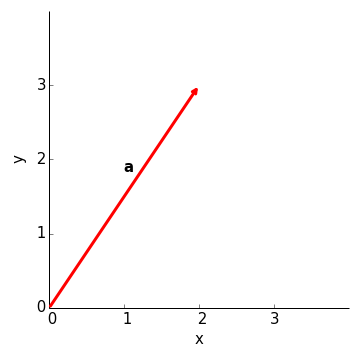
\includegraphics[width=\textwidth]{figure1.png}
\caption{
	$\mathbf{a} = \left(
	\begin{array}{c}
	2\\
	3\\
	\end{array}
	\right)$}

\label{Geometry}
\end{center}
\end{figure}
\end{columns}
\end{frame}

%------------------------------------------------
\begin{frame}
\begin{block}{Q}
Scalar or vector?
\end{block}

\begin{block}{examples}
Speed, Weight, Velocity, Force?
\end{block}
\end{frame}
%------------------------------------------------
\section{Vector addition and scalar multiplication}
\frametitle{Addition and subtraction}

\begin{frame}
Given two vectors $$\mathbf{v} = \left(
	\begin{array}{c}
	a\\
	b\\
	\end{array}
	\right)$$
and
	$$\mathbf{w} = \left(
	\begin{array}{c}
	c\\
	d\\
	\end{array}
	\right)$$\\
	Vector addition is then simply
	
	$$\mathbf{v+w} = \left(
	\begin{array}{c}
	a+c\\
	b+d\\
	\end{array}
	\right)$$\\
	
	similarly:
	$$\mathbf{v-w} = \left(
	\begin{array}{c}
	a-c\\
	b-d\\
	\end{array}
	\right)$$
	
	
\end{frame}
%------------------------------------------------
\begin{frame}
\frametitle{The geometry of vector addition}
If 
	$\mathbf{v} = \left(
	\begin{array}{c}
	1\\
	3\\
	\end{array}
	\right)$ 
and 
	$\mathbf{w} = \left(
	\begin{array}{c}
	2\\
	1\\
	\end{array}
	\right)$, draw $\mathbf{v+w} $

\begin{figure}[htbp]
\begin{center}
 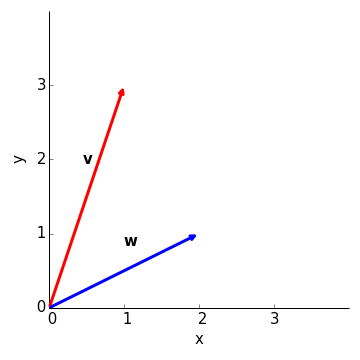
\includegraphics[width=0.55\textwidth]{figure2a.png}
\caption{}


\end{center}
\end{figure}

	
\end{frame}
%------------------------------------------------
\begin{frame}
$$\mathbf{v+w} = \left(
	\begin{array}{c}
	1+2\\
	3+1\\
	\end{array}
	\right) 
	= 
	\left(
	\begin{array}{c}
	3\\
	4\\
	\end{array}
	\right)$$\\



\end{frame}
%------------------------------------------------
\begin{frame}

\begin{figure}[htbp]
\begin{center}
 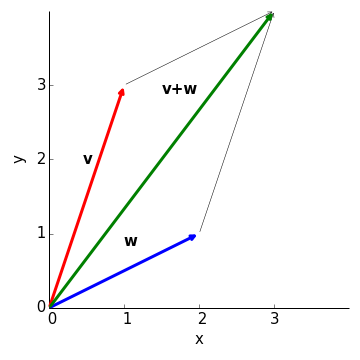
\includegraphics[width=0.65\textwidth]{figure2b.png}
\caption{}
\end{center}
\end{figure}

\end{frame}
%------------------------------------------------

\begin{frame}
\frametitle{Vector addition}
Question number 2 of the preparatory questions:\\[1cm]
Let $P = (-2,-1)$, $Q = (-3,3)$, and $R = (-1,-4)$ in the xy-plane.\\
\begin{itemize}
\item Draw these vectors: $\mathbf{v}$ joining $P$ to $Q$; $\mathbf{w}$  joining $Q$ to $R$, and $\mathbf{u}$  joining $R$ to $P$
\item What are the component vectors of $\mathbf{v}$, $\mathbf{w}$ and $\mathbf{u}$?
\item What is $\mathbf{v + w + u}$?
\end{itemize}
[ex 9. p. 13]
\end{frame}
%------------------------------------------------

\begin{frame}
\frametitle{Scalar multiplication}

if we have a vector $$\mathbf{v} = \left(
	\begin{array}{c}
	a\\
	b\\
	\end{array}
	\right)$$\\[1cm]
then the scalar multiplication (with scalar $s$) equals:
$$s\mathbf{v} = \left(
	\begin{array}{c}
	sa\\
	sb\\
	\end{array}
	\right)$$
\end{frame}
%------------------------------------------------
\begin{frame}
\frametitle{The geometry of scalar multiplication}

\begin{figure}[htbp]
\begin{center}
 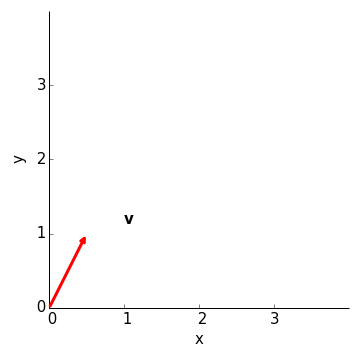
\includegraphics[width=0.65\textwidth]{figure3a.png}
\caption{}
\end{center}
\end{figure}

\end{frame}

%------------------------------------------------
\begin{frame}
\frametitle{scalar multiplication}

\begin{figure}[htbp]
\begin{center}
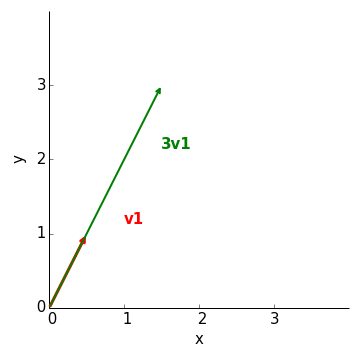
\includegraphics[width=0.65\textwidth]{figure3b.png}
\caption{}
\end{center}
\end{figure}

\end{frame}
%------------------------------------------------
\section{Vector inner and outer products}
\begin{frame}
\frametitle{Vectors: the inner product or dot product}
The inner product has some nice features - it is often used to quantify the angle between two vectors. First let's define the inner product of $\mathbf{v}$ and $\mathbf{w}$.


$$ \mathbf{v} \cdot \mathbf{w} = v_1w_1 + v_2w_2 + v_3w_3$$\\[1cm]
The inner product of two  {\color<1>[rgb]{1,0,0}{vectors}} is thus a  {\color<1>[rgb]{0.5,0.8,0.1}{scalar quantity}}

\end{frame}
%------------------------------------------------
\begin{frame}
Important concepts in vector calculus are the \mathbf{length} of a vector. From the Pythagorean theorem if easily follows that the length of vector
\begin{columns}[c]
\column{.45\textwidth} 

	$$\mathbf{a} = \left(
		\begin{array}{c}
		a_1\\
		a_2\\
		a_3\\
		\end{array}
	\right)$$
is $$|| \mathbf{a}  || = \sqrt{a_{1}^{2} + a_{2}^{2} + a_{3}^{2} }$$
This quality is often called the norm of  \mathbf{a}. This can also be used to calculate the distance between the endpoints of e.g., \mathbf{a} and \mathbf{b} as $||\mathbf{a}-\mathbf{b}||$.    

\column{.5\textwidth} 
\begin{figure}[htbp]
\begin{center}
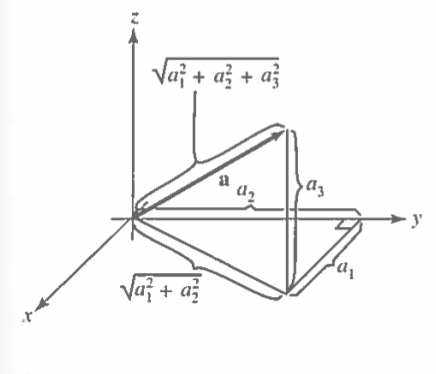
\includegraphics[width=1.1\textwidth]{fig_pyth.png}
\end{center}
\end{figure}
\end{columns}
\end{frame}

%------------------------------------------------
\begin{frame}
So, the length --or norm-- of a vector \mathbf{a} is equal to 
$$|| \mathbf{a}  ||  = \sqrt{a_{1}^{2} + a_{2}^{2} + a_{3}^{2}}$$ 

Since $\mathbf{a} \cdot \mathbf{a} = a_{1}^{2} + a_{2}^{2} + a_{3}^{2}$, it follows that $$|| \mathbf{a} || = \sqrt{ \mathbf{a} \cdot \mathbf{a} } = \left( \mathbf{a} \cdot \mathbf{a} \right)^{1/2}$$

Vectors with norm 1 are called unit vectors. It follows that for any (nonzero) vector, the unit vector can be obtained by dividing \mathbf{a}  by  $|| \mathbf{a} ||$ and is also called a normalised \mathbf{a}. \\[1cm]
\end{frame}

%------------------------------------------------
\begin{frame}

One application of the inner product is that it can be used to determine the angle between two vector. How? Let's see.
Remember the cosine rule? 
\begin{columns}[c]
\column{.45\textwidth} 
$$ c^2 = a^2 + b^2 - 2ab\cos{C}$$


\column{.5\textwidth} 
\begin{figure}[htbp]
\begin{center}
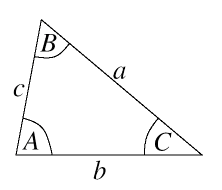
\includegraphics[width=0.8\textwidth]{abc.png}
\caption{}
\end{center}
\end{figure}
\end{columns}
\end{frame}

%------------------------------------------------
\begin{frame}
So, by knowing the length of the three sides of a triangle we can obtain the angle between each pair of vectors; we know the length of the two vectors $\mathbf{a}$ and  $\mathbf{b}$. We also know the distance between them: 
$||\mathbf{b}-\mathbf{a}||$.  Plugging these values into the cosine rule:
$$ c^2 = a^2 + b^2 - 2ab\cos{\theta}$$
$$ ||\mathbf{b}-\mathbf{a}||^2 = ||\mathbf{a}||^2 + ||\mathbf{b}||^2  - 2||\mathbf{a}||||\mathbf{b}||\cos{\theta}$$
Since $||\mathbf{b}-\mathbf{a}||  = \left( \mathbf{b}-\mathbf{a} \right) \cdot  \left( \mathbf{b}-\mathbf{a} \right)$, 
 $||\mathbf{a}||  = \mathbf{a} \cdot   \mathbf{a}$ and 
 $||\mathbf{b}||  = \mathbf{b} \cdot   \mathbf{b}$, we can rewrite this as:
 $$\left( \mathbf{b}-\mathbf{a} \right) \cdot  \left( \mathbf{b}-\mathbf{a} \right) = \mathbf{a} \cdot   \mathbf{a} + \mathbf{b} \cdot   \mathbf{b} - 
 2  ||\mathbf{a}||  ||\mathbf{b}|| \cos \theta$$
 
\end{frame}
%------------------------------------------------
\begin{frame}


Now 
$$\left( \mathbf{b}-\mathbf{a} \right) \cdot  \left( \mathbf{b}-\mathbf{a} \right)  = \mathbf{b} \cdot \left( \mathbf{b}-\mathbf{a} \right) - \mathbf{a} \cdot \left( \mathbf{b}-\mathbf{a} \right)$$
$$ = \mathbf{b} \cdot \mathbf{b} - \mathbf{b} \cdot \mathbf{a} - \mathbf{a} \cdot \mathbf{b} + \mathbf{a} \cdot \mathbf{a} $$
$$ = \mathbf{a} \cdot \mathbf{a} + \mathbf{b} \cdot \mathbf{b} - 2 \mathbf{a} \mathbf{b} $$
Thus
$$ = \mathbf{a} \cdot \mathbf{a} + \mathbf{b} \cdot \mathbf{b} - 2 \mathbf{a} \mathbf{b}  = = \mathbf{a} \cdot \mathbf{a} + \mathbf{b} \cdot \mathbf{b}  - 2 ||\mathbf{a}||  ||\mathbf{b}|| \cos \theta $$
That is,
$$ = \mathbf{a} \cdot \mathbf{b} =  ||\mathbf{a}||  ||\mathbf{b}|| \cos \theta$$

\end{frame}
%------------------------------------------------
\begin{frame}
\begin{columns}[c]
\column{.45\textwidth} 
So, the two vector define the angle $\theta$ between them by
$$ \theta = cos^{-1}\left(\frac{\mathbf{a} \cdot \mathbf{b}}{\Vert \mathbf{a}\Vert  \Vert \mathbf{b} \Vert} \right)$$

\column{.5\textwidth} 
Exercise [ex 4, p 29]:
\begin{figure}[htbp]
\begin{center}
 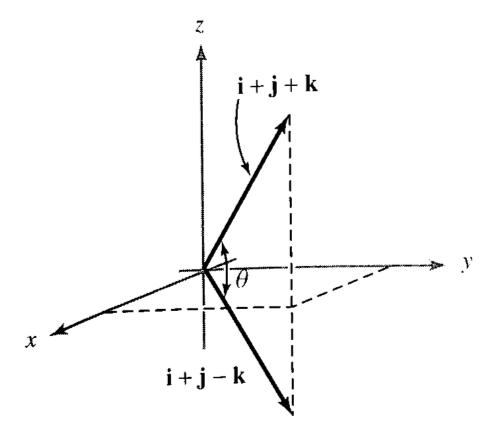
\includegraphics[width=\textwidth]{angle_vector.png}
\caption{}
\end{center}
\end{figure}
\end{columns}
\end{frame}

%------------------------------------------------

\begin{frame}
\frametitle{Practical application: physics}
\begin{block}{Q}
A bird is flying in a straight line with velocity vector 10 \mathbf{i} +  6 \mathbf{j} +  \mathbf{k}  (in km/h). Suppose that $\left(x,y\right)$ are its coordinates on the ground and $z$ its height above the ground. [ex 11, p 35]
\begin{itemize}
\item If the bird is at $(1,2,3)$ at a certain moment, where is it 1h later?
\item How many second does it take the bird to climb 10m?
\end{itemize}

\end{block}  
\end{frame}

%------------------------------------------------
\begin{frame}
\frametitle{Orthogonal projection}
\begin{columns}[c]
\column{.45\textwidth} 
The orthogonal projection $\mathbf{p} $ of $\mathbf{w}$ on $\mathbf{v}$  is the vector whose tip is obtained by dropping a perpendicular line to the line $l$ (along v) from the top of $\mathbf{w}$. We can obtain the projection as:
$$  \mathbf{p} =\frac{ \mathbf{v} \cdot  \mathbf{w}}{\Vert \mathbf{v} \Vert^2}  \mathbf{v} $$

\column{.5\textwidth} 
\begin{figure}[htbp]
\begin{center}
 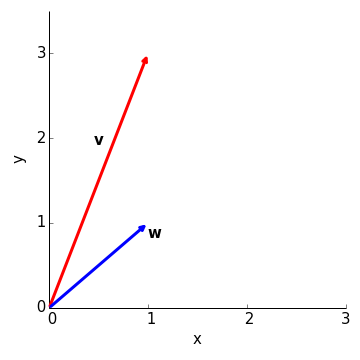
\includegraphics[width=\textwidth]{figure4a.png}
\caption{}
\end{center}
\end{figure}
\end{columns}
\end{frame}

%------------------------------------------------
\begin{frame}
\begin{columns}[c]
\column{.45\textwidth} 

So, 
	$\mathbf{v} = \left(
		\begin{array}{c}
		1\\
		3\\
		\end{array}
	\right)$

and 
	$\mathbf{w} = \left(
		\begin{array}{c}
		1\\
		1\\
		\end{array}
	\right)$\\
	

$$\mathbf{v} \cdot  \mathbf{w} = 1*1 + 3 *1 = 4 $$
$$\Vert \mathbf{v} \Vert^2 = 1^2 + 3^2 = 10 $$
$$  \mathbf{p} =\frac{\mathbf{v} \cdot  \mathbf{w}} {\Vert \mathbf{v} \Vert^2} \mathbf{v} =   \frac{4}{10} \left(
		\begin{array}{c}
		1\\
		3
		\end{array}
		\right)		
		= \left(
		\begin{array}{c}
		0.4\\
		1.2
		\end{array}
		\right)$$

\column{.45\textwidth} 
\begin{figure}[htbp]
\begin{center}
 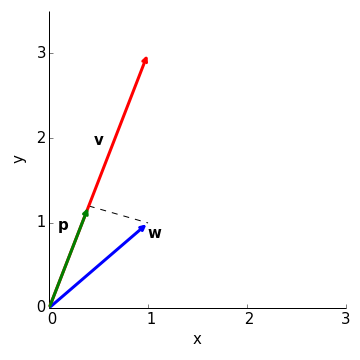
\includegraphics[width=\textwidth]{figure4b.png}
\caption{}
\end{center}
\end{figure}
\end{columns}
\end{frame}


%------------------------------------------------


\begin{frame}
\frametitle{Vectors: determinants and the cross-product}
So far we've encountered
\begin{itemize}
\item vector addition
\item scalar-product
\item the inner-product closely related to the length of a vector and used to calculate the angle between vectors.
\end{itemize}
In what follows, we'll discuss another property of vector calculus: {\color<1>[rgb]{1,0,0}{the outer product}}

\end{frame}
%------------------------------------------------

\begin{frame}
\frametitle{Vectors: determinants}
Previously, we've encountered the inner product of two vectors that generated a scalar. In what follows we define a product of vectors that is a vector. Given two vectors $\mathbf{v}$ and $\mathbf{w}$, we can obtain a third vector $\mathbf{v} \times \mathbf{w}$, the cross-product of $\mathbf{v}$ and $\mathbf{w}$. This vector will have the (pleasing) geometrical property that is it perpendicular to the plane spanned by $\mathbf{v}$ and $\mathbf{w}$.\\[0.5cm]

First, let's define a 2 x 2 matrix $\mathbf{M}$ as 
$$  \mathbf{M} = \[ \left( \begin{array}{cc}
a_{11} & a_{12} \\
a_{21} & a_{22} \end{array} \right)\] $$\\
the determinant is then defined as:
$$ 
\left| \mathbf{M} \right| =
 \left| \begin{array}{cc}
a_{11} & a_{12} \\
a_{21} & a_{22} \end{array} \right| = a_{11}a_{22} - a_{12}a_{21}
$$


\end{frame}
%------------------------------------------------
\begin{frame}
or, with a 3 x 3 matrix:
$$ 
 \left| \begin{array}{ccc}
{\color<1>[rgb]{1,0,0}{a_{11}}} & a_{12} & a_{13} \\
a_{21} & {\color<1>[rgb]{1,0,0}{a_{22}}}  & {\color<1>[rgb]{1,0,0}{a_{23}}}  \\
a_{31} & {\color<1>[rgb]{1,0,0}{a_{32}}}  & {\color<1>[rgb]{1,0,0}{a_{33}}} 
\end{array} \right| = {\color<1>[rgb]{1,0,0}{a_{11}}}
\left| \begin{array}{cc}
{\color<1>[rgb]{1,0,0}{a_{22}}} & {\color<1>[rgb]{1,0,0}{a_{23}}} \\
{\color<1>[rgb]{1,0,0}{a_{32}}}  & {\color<1>[rgb]{1,0,0}{a_{33}}}  
\end{array} \right|  -  a_{12}
 \left| \begin{array}{cc}
a_{21} & a_{23} \\
a_{31} & a_{33} \end{array} \right| + a_{13}
\left| \begin{array}{cc}
a_{21} & a_{22} \\
a_{31} & a_{32} \end{array} \right| $$
\end{frame}
%------------------------------------------------
\begin{frame}
or, with a 3 x 3 matrix:
$$ 
 \left| \begin{array}{ccc}
a_{11} &  {\color<1>[rgb]{0.1,0.95,0.1}{a_{12}}}  & a_{13} \\
 {\color<1>[rgb]{0.1,0.95,0.1}{a_{21}}} &  a_{22} &  {\color<1>[rgb]{0.1,0.95,0.1}{a_{23}}}  \\
 {\color<1>[rgb]{0.1,0.95,0.1}{a_{31}}} &  a_{32} &  {\color<1>[rgb]{0.1,0.95,0.1}{a_{33}}} 
\end{array} \right| = a_{11}  
\left| \begin{array}{cc}
a_{22} & a_{23} \\
a_{32} & a_{33} \end{array} \right|  -  {\color<1>[rgb]{0.1,0.95,0.1}{a_{12}}}  
 \left| \begin{array}{cc}
 {\color<1>[rgb]{0.1,0.95,0.1}{a_{21}}}  &  {\color<1>[rgb]{0.1,0.95,0.1}{a_{23}}}  \\
 {\color<1>[rgb]{0.1,0.95,0.1}{a_{31}}}  &  {\color<1>[rgb]{0.1,0.95,0.1}{a_{33}}}  \end{array} \right| + a_{13}
\left| \begin{array}{cc}
a_{21} & a_{22} \\
a_{31} & a_{32} \end{array} \right| $$
\end{frame}

%------------------------------------------------

\begin{frame}
the determinant is then defined as:
$$ 
 \left| \begin{array}{cc}
a_{11} & a_{12} \\
a_{21} & a_{22} \end{array} \right| = a_{11}a_{22} - a_{12}a_{21}
$$

or, with a 3 x 3 matrix:
$$ 
 \left| \begin{array}{ccc}
a_{11} & a_{12}  &  {\color<1>[rgb]{0.1,0.1,0.9}{a_{13}}} \\
 {\color<1>[rgb]{0.1,0.1,0.9}{a_{21}}} &  {\color<1>[rgb]{0.1,0.1,0.9}{a_{22}}}  & a_{23}   \\
 {\color<1>[rgb]{0.1,0.1,0.9}{a_{31}}} &  {\color<1>[rgb]{0.1,0.1,0.9}{a_{32}}}  & a_{33} 
\end{array} \right| = a_{11}  
\left| \begin{array}{cc}
a_{22} & a_{23} \\
a_{32} & a_{33} \end{array} \right|  -  a_{12}
 \left| \begin{array}{cc}
a_{21} & a_{23} \\
a_{31} & a_{33} \end{array} \right| + {\color<1>[rgb]{0.1,0.1,0.9}{a_{13}}}
\left| \begin{array}{cc}
{\color<1>[rgb]{0.1,0.1,0.9}{a_{21}}} &  {\color<1>[rgb]{0.1,0.1,0.9}{a_{22}}} \\
{\color<1>[rgb]{0.1,0.1,0.9}{a_{31}}} &  {\color<1>[rgb]{0.1,0.1,0.9}{a_{32}}}
 \end{array} \right| $$
\end{frame}

%------------------------------------------------
\begin{frame}
This looks like a lot of work to get another vector, but there is some history and application to it:
\begin{itemize}
\item Linear equations and Cramer's rule (remember)
\item 2D: The area of the parallelogram defined by two vectors 
\item 3D: The volume of a parallelepiped
%\item Find the normal-vector, the vector that is orthogonal to any vector in the plane spanned by vectors a and b.
\end{itemize}

\end{frame}
%------------------------------------------------
\begin{frame}
\frametitle{Cramer's law to linear equations (1750!)}
Say we have a system of equations:
%source http://www.purplemath.com/modules/cramers.htm
$$
\begin{array}{ccc}
2x + y + z &=& 3\\
x-y-z &=& 0\\
x + 2y + z &=& 0
\end{array}$$\\
Or rewritten like $A x = b$,
$$\left(\begin{array}{ccc}
2 & 1 & 1\\
1 & -1 & -1\\
1 & 2 & 1 \end{array} \right)
\left( \begin{array}{c}
x \\
y \\
z  \end{array} \right) = 
\left( \begin{array}{c}
3 \\
0 \\
0 \end{array} \right)$$
This system can be solved (i.e., finding the values of $x, y, z$ for which all three equations make sense) by using \emph{determinants}.
\end{frame}
%------------------------------------------------

\begin{frame}
\frametitle{Cramer's law : step 1}

First find the determinant of the equations:
$$ \Delta =  \left| \begin{array}{ccc}
a_{11} & a_{12} & a_{13} \\
a_{21} & a_{22} & a_{23} \\
a_{31} & a_{32} & a_{33} \end{array} \right| = 
\left| \begin{array}{ccc}
2 & 1& 1  \\
1 & -1 & -1 \\
1 & 2 & 1 \end{array} \right| = 
$$
$$ 2 
\left| \begin{array}{cc}
-1 & -1  \\
2 & 1 \end{array} \right| 
 - 1
\left| \begin{array}{cc}
1 & -1 \\
1 & 1 \end{array} \right| + 1
\left| \begin{array}{cc}
1& -1 \\
1 & 2 \end{array} \right| = ...
$$
%
\end{frame}
%------------------------------------------------

\begin{frame}
\frametitle{Cramer's law : step 2}
The next step is to plug the answer vector (the vector describing the results) into the three separate determinants -- these are going to be used to determine the solution to the system of equations.
So,
$$\Delta_{x} = 
\left| \begin{array}{ccc}
{\color<1>[rgb]{1,0,0}{3}}  & 1& 1  \\
{\color<1>[rgb]{1,0,0}{0}}  & -1 & -1 \\
{\color<1>[rgb]{1,0,0}{0}}  & 2 & 1 \end{array} \right| = 3
$$

$$\Delta_{y} = 
\left| \begin{array}{ccc}
2 & {\color<1>[rgb]{1,0,0}{3}}  & 1  \\
1 & {\color<1>[rgb]{1,0,0}{0}}  & -1 \\
1 & {\color<1>[rgb]{1,0,0}{0}}  & 1 \end{array} \right| = -6
$$

$$\Delta_{z} = 
\left| \begin{array}{ccc}
2 & 1  & {\color<1>[rgb]{1,0,0}{3}}\\
1 & -1 & {\color<1>[rgb]{1,0,0}{0}}\\
1 & 2  & {\color<1>[rgb]{1,0,0}{0}}\end{array} \right| = 9
$$

\end{frame}
%------------------------------------------------

\begin{frame}
\frametitle{Cramer's law : step 3}
The final step to the solution is Cramer's rule:

$$ x = \frac{\Delta_{x}}{\Delta} = \frac{3}{3} = 1$$
$$ y = \frac{\Delta_{y}}{\Delta} = \frac{-6}{3} = -2$$
$$ z = \frac{\Delta_{z}}{\Delta} = \frac{9}{3} = 3$$

Exercise 1: check whether the above solution is a valid one. \\


\end{frame}
%------------------------------------------------
\begin{frame}
Exercise 2: check whether this method works for the following\\

$$
\begin{array}{ccc}
2x + y + z &=& 3\\
x+y/2 + z/2 &=& 3/2\\
x + 2y + z &=& 0
\end{array}$$

\end{frame}


%------------------------------------------------
\begin{frame}
\frametitle{Geometry of 2x2 determinants}
Let $\mathbf{a} = a_1 \mathbf{i} + a_2 \mathbf{j}$ and $\mathbf{b} = b_1 \mathbf{i} + b_2 \mathbf{j}$ be two vectors in the (i,j) plane. Then the cross-product can be described as a determinant:

$$\mathbf{a}  \times \mathbf{b} =  
\left| \begin{array}{ccc}
\mathbf{i} & \mathbf{j} & \mathbf{k}\\
a_1 & a_2 & 0\\
b_1 & b_2 & 0
\end{array}
\right| =  
\left| \begin{array}{cc}
a_1 & a_2 \\
b_1 & b_2 
\end{array} \right| \mathbf{k}$$

This is a very interesting property: it indicates that the area  $ || \mathbf{a}  \times \mathbf{b} || $ equals the absolute value of the determinant.
$$ || \mathbf{a}  \times \mathbf{b} ||  = | a_1b_2 - a_2b_1 | $$

%
%
%
%Then it turns out that the determinant of the cross-product is equal to the area of the parallelogram spanned by $\mathbf{a}$ and $\mathbf{b}$. So:
\end{frame}

\begin{frame}
\frametitle{Geometry of 2x2 determinants}
It can also be determined by determining 

$$|| \mathbf{a} \times \mathbf{b}|| = || \mathbf{a} || ||\mathbf{b}|| \sin{\theta}$$    
\begin{figure}[htbp]
\begin{center}
 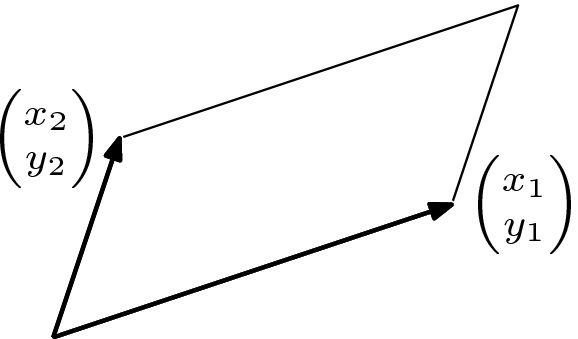
\includegraphics[width=0.7\textwidth]{parallelogram.png}
\caption{}
\end{center}
\end{figure}
\end{frame}
%------------------------------------------------
\begin{frame}
\frametitle{Geometry of 3x3 determinants}
Let $\mathbf{a} = a_1 \mathbf{i} + a_2 \mathbf{j} + a_3 \mathbf{k}$  and $\mathbf{b} = b_1 \mathbf{i} + b_2 \mathbf{j} + b_3 \mathbf{k}$, and   $\mathbf{c} = c_1 \mathbf{i} + c_2 \mathbf{j} + c_3 \mathbf{k}$ be three vectors in the 
$(i,j,j)$ plane. Then the absolute value of the determinant $D$ is the volume of the parallelpiped.
\begin{columns}[c]
\column{.45\textwidth} 

$$D =  
\left| \begin{array}{ccc}
a_1 & a_2 & a_3\\
b_1 & b_2 & b_3\\
c_1 & c_2 & c_3
\end{array}
\right|$$
\column{.5\textwidth} 
\begin{figure}[htbp]
\begin{center}
 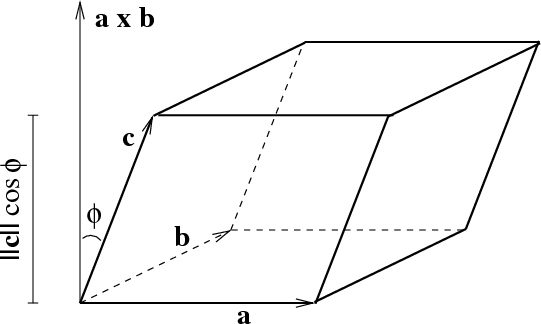
\includegraphics[width=\textwidth]{volume_parallelepiped.png}
\caption{}
\end{center}
\end{figure}
\end{columns}
\end{frame}

\section{summary}
\begin{frame}
\frametitle{summary}
Today we've encountered vectors and various related properties:
\begin{itememize}
\item scalar multiplication
\item vector addition
\item inner product  $\mathbf{a} \cdot  \mathbf{b}$
\item outer product $\mathbf{a} \times \mathbf{b}$
\end{itemize}

Next time,  we'll cover some more applications
\end{frame}

\begin{frame}
\frametitle{bonus infinite sum}
\begin{block}{Q}
What is the sum of all natural numbers $1+2+3 ... \inf$?
$$\sum_n^{\inf}n = - \frac{1}{12}$$
\end{block}
\end{frame}

\begin{frame}
\Huge{\centerline{Questions}}
\end{frame}

%----------------------------------------------------------------------------------------



\end{document} 